\section{Abbildungen}
%=============================

\textit{Latex} unterst�tzt generell die Formate \textit{*.jpeg}, \textit{*.png} und \textit{*.pdf}.
Handelt es sich z.B. um Strichgrafiken oder skalierbare Farbfl�chen, sollte \textit{*.pdf} die erste Wahl sein,
da dieses Format sich ohne Qualit�tsverlust skalieren l�sst.

\subsection{Eine erste Abbildung}

\blindtext
\begin{figure}[htbp] 
  \centering
  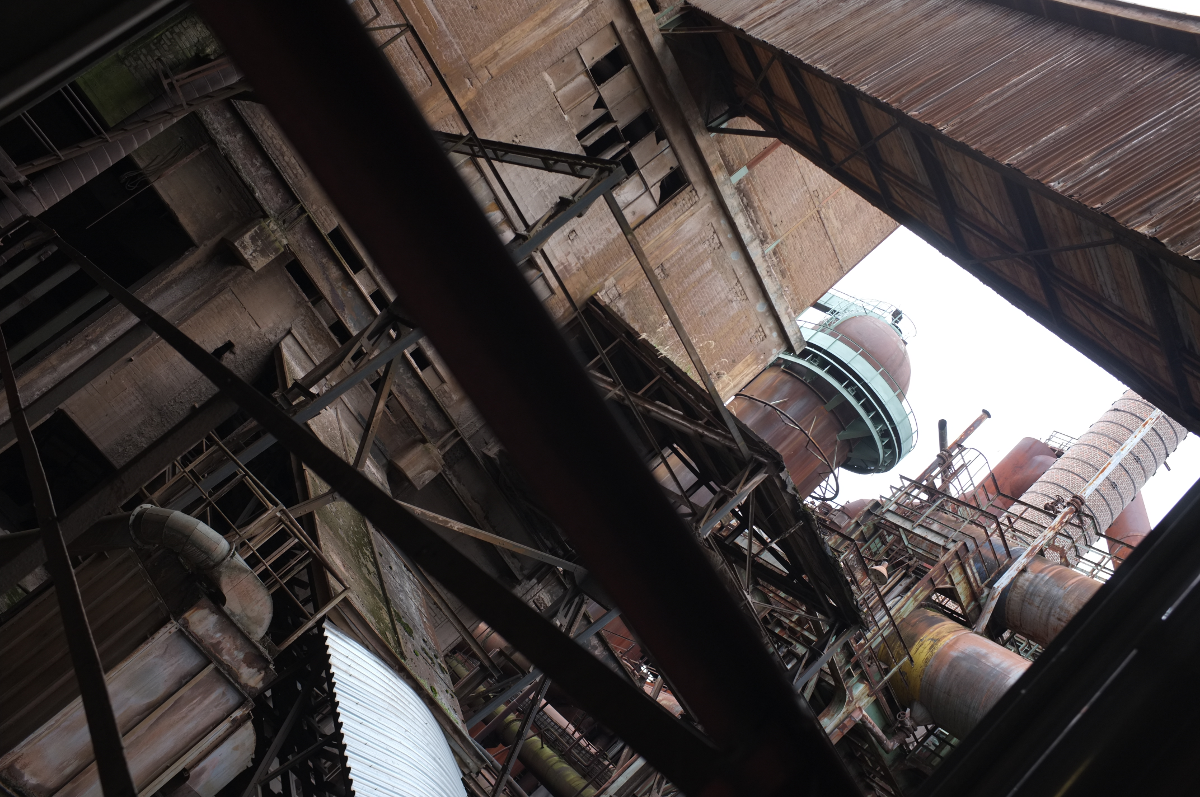
\includegraphics[width=0.7\textwidth]{Examples/example_5.png}
  \caption{Erstes Bild, V�lklinger H�tte}
  \label{fig:Huette}
\end{figure}

\subsection{Es geht besser}

Abbildung \ref{fig:Huette} ist zwar ganz nett anzusehen, aber vielleicht s�he es eleganter aus, wenn die Abbildung 
von unserem Textabschnitt umflossen wird.


\blindtext
\begin{wrapfigure}{l}{0.5\textwidth}
  \centering
  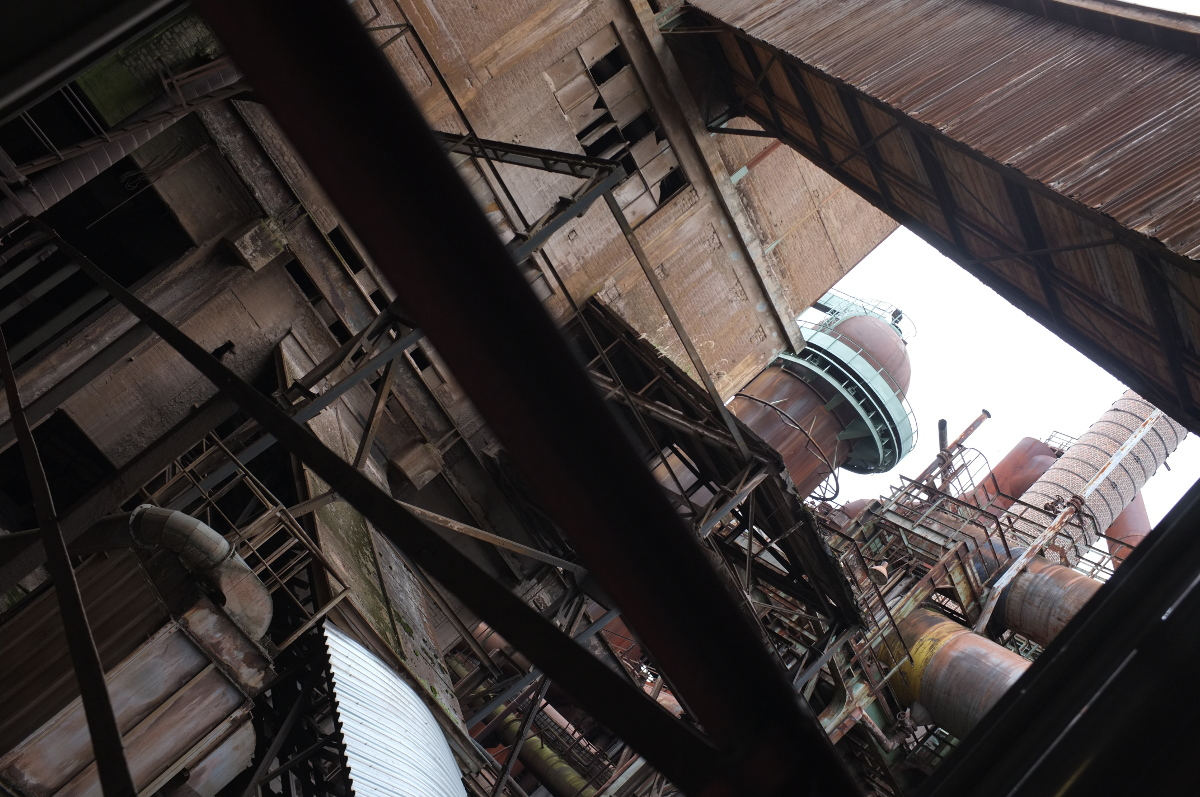
\includegraphics[width=0.5\textwidth]{Examples/example_5.jpg}
  \caption{V�lklinger H�tte, *.jpg}
  \label{fig:Huette2}
\end{wrapfigure}
\blindtext
\blindtext

\subsection{Mehrere Abbildungen nebeneinander}

Es ist ebenso m�glich mehrere Abbildungen nebeneinander zu setzen, wie in Abbildung \ref{fig:Beide} zu sehen ist.

\begin{figure}
  \subfloat[Erstes ...]{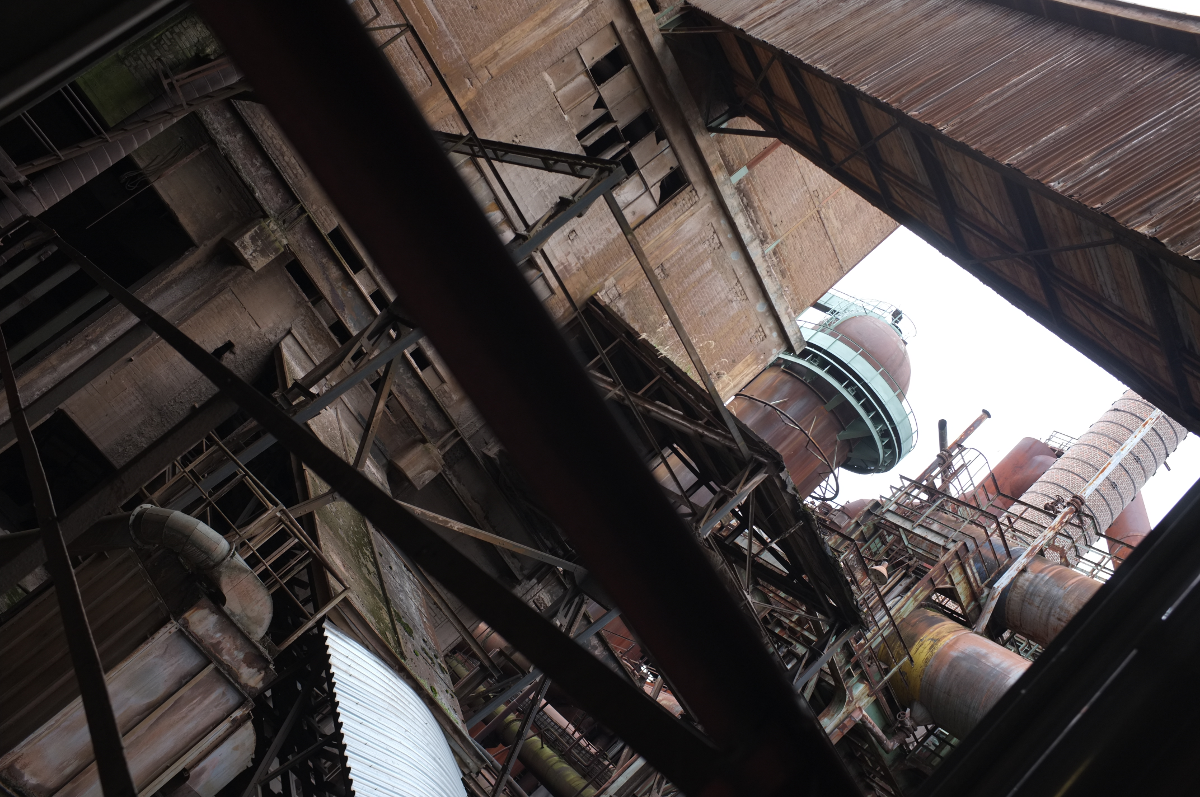
\includegraphics[width=0.49\textwidth]{Examples/example_5.png}}\hfill
  \subfloat[... und zweites Bild]{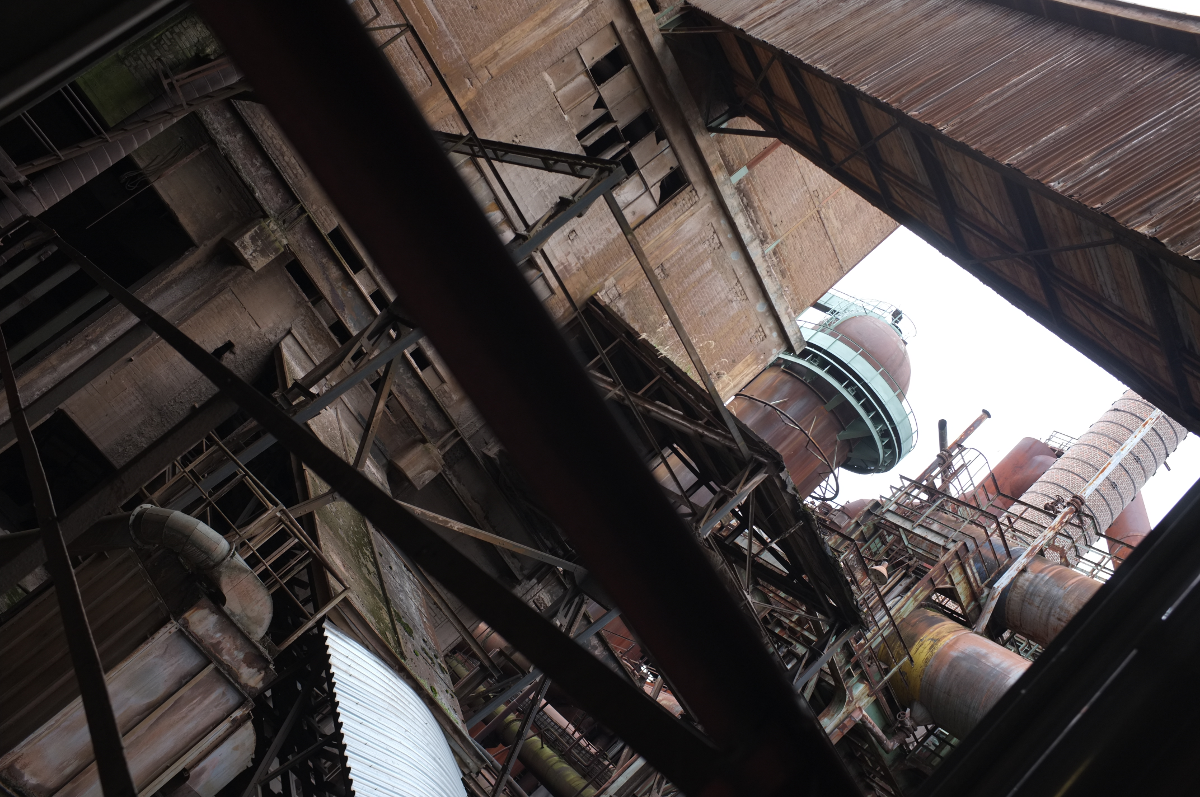
\includegraphics[width=0.49\textwidth]{Examples/example_5.png}}
  \caption{Abbildung \ref{fig:Huette} und \ref{fig:Huette2} nebeneinander}
  \label{fig:Beide}
\end{figure}

